\documentclass[notheorems, 9pt]{beamer}

% Packages with options
\usepackage[english]{babel}
\usepackage[mathscr]{euscript}
\usepackage[utf8]{inputenc}

% Primary Packages
\usepackage{amsbsy, amsmath, amssymb, amsthm, bm, commath, chngcntr, dsfont, econometrics, gensymb, graphicx, IEEEtrantools, longtable, marginnote, mathrsfs, mathtools, mdframed, natbib, parskip, pgf, setspace, subfigure, tabularx, textcomp, tikz}

% Rest of the setup is in the "setup_beamer" package
\usepackage{setup_beamer}

% Title, Author, Institute
\title{Econ 103: Topics in Single Linear Regression}
\author{Manu Navjeevan}
\institute{UCLA}

%%%%%%%%%%%%%%%%%%%%%%%%%%%%%%%%%%%%%%%%%%%%%

\begin{document}
\frame{\titlepage}

%NOTE: Cover: R^2, Inference on Linear Combinations, Forecast Error, Heteroskedasticity

\begin{frame}{Content Outline} 
	\label{frame:content-outline}
	\ucla{Advanced Inference Topics}
	\begin{itemize}
		\item Inference on Linear Combinations of Parameters
		\item Heteroskedasticity
	\end{itemize}
	\ucla{Evaluating our Model}
	\begin{itemize}
		\item Prediction
		\item \(R^2\) and goodness of fit
	\end{itemize}
	\ucla{Modeling Choices}
	\begin{itemize}
		\item How do results change if we apply linear transformations?
		\item Useful non-linear transformations of \(X\) and \(Y\)
	\end{itemize}
\end{frame}

\section{Advanced Inference Topics}
%NOTE: Linear combinations, forecast error, heteroskedasticity
\begin{frame}{Inference: Linear Combinations of Parameters} 
	\label{frame:lc1}
	Recall that, approximately for large \(n\)
	\begin{align*}
		\sqrt{n}(\ucla{\hat\beta_0} - \ucla{\beta_0}) \sim N\left(0, \E[X^2]\sigma_\eps^2/\sigma_X^2 \right),\;\;
		\sqrt{n}(\ucla{\hat\beta_1} - \ucla{\beta_1}) \sim N\left(0, \sigma_\eps^2/\sigma_X^2\right)
	\end{align*}
	and \(\sigma_{\beta_{01}} = \Cov(\sqrt{n}\{\ucla{\hat\beta_0}-\ucla{\beta_0}\},\sqrt{n}\{\ucla{\hat\beta_1}-\ucla{\beta_1}\}) = -\E[X]\frac{\sigma_\eps^2}{\sigma_X^2}.\)
	\onslide<2->
	\vspace{0.5cm}

	These results were also often presented in the following equivalent manners
	\begin{align*}
		\frac{\ucla{\hat\beta_0}-\ucla{\beta_0}}{\sigma_{\beta_0}/\sqrt{n}}\sim N(0,1) &\andbox \ucla{\hat\beta_0} \sim N(\ucla{\beta_1},\sigma_{\beta_0}^2/n) \\
		\frac{\ucla{\hat\beta_1}-\ucla{\beta_1}}{\sigma_{\beta_1}/\sqrt{n}}\sim N(0,1) &\andbox \ucla{\hat\beta_1}\sim N(\ucla{\beta_1},\sigma_{\beta_1}^2/n) 
	\end{align*}
	where \(\sigma_{\beta_0}^2 = \E[X^2]\sigma_{\eps^2}/\sigma_X^2\) and \(\sigma_{\beta_1}^2 = \sigma_\eps^2/\sigma_X^2\).
	 \begin{itemize}
		\item<3-> Also went over how to estimate these variances
	\end{itemize}
	
\end{frame}
\begin{frame}{Inference: Linear Combinations of Parameters} 
	\label{frame:lc}
	In the last lecture, we used these distributional results to compute objects like 
	\[
		\Pr\left(|\ucla{\hat\beta_1}| > 5 \mid \ucla{\beta_1} = 0\right)
	.\] 
	which in turn were useful for hypothesis testing
	\[
		\green{H_0}:\ucla{\beta_1}= 0\vsbox \red{H_1}:\ucla{\beta_1} \neq 0
	.\] 
\end{frame}
\begin{frame}{Inference: Linear Combinations of Parameters} 
	\label{frame:lc2}
	However, often we want to preform inference not just on one parameter, but on a linear combination of parameters, i.e we want to test 
	\[
		\green{H_0}:\ucla{\beta_0} + 5\ucla{\beta_1} = 0\vsbox \red{H_1}:\ucla{\beta_0} + 5\ucla{\beta_1}\neq 0
	.\] 
	\onslide<2->
	This is useful, for example, if we are trying to test something like 
	\[
		\green{H_0}:\E[Y|X=5] = 0\vsbox\red{H_1}:\E[Y|X=5]\neq 0
	\] 
	and we view the linear regression model \(Y = \ucla{\beta_0} + \ucla{\beta_1}X + \eps\) as a way of approximating the conditional mean function \(\E[Y|X=x]\). 
\end{frame}
\begin{frame}{Inference: Linear Combinations of Parameters} 
	\label{frame:lc3}
	In order to test such a hypothesis we want to know the distribution of a linear combination of our model parameters. That is, for \(\lambda = a\ucla{\beta_0} + b\ucla{\beta_1}\) we would like to know the approximate distribution of
	\[
	    \hat\lambda = a\ucla{\hat\beta_0} + b \ucla{\hat\beta_1}
	\] 
	so that we can calculate objects like \(\Pr(|\hat\lambda| > 0.5 \mid \lambda = 0)\).
	\onslide<2->

	Note that
	\begin{align*}
		\sqrt{n}\left(\hat\lambda - \lambda\right) &= \sqrt{n}\left(a\ucla{\hat\beta_0} + b\ucla{\hat\beta_1} - a\ucla{\beta_0} - b \ucla{\beta_1}\right) \\
		&= a\sqrt{n}\left(\ucla{\hat\beta_0} - \ucla{\beta_0}\right) + b\sqrt{n}\left(\ucla{\hat\beta_1}-\ucla{\beta_1}\right)
	.\end{align*} 
	and that we know the (joint) distribution of \( \sqrt{n}(\ucla{\hat\beta_0}-\ucla{\beta_0})\) and \(\sqrt{n}(\ucla{\hat\beta_1}-\ucla{\beta_1})\).
\end{frame}
\begin{frame}{Inference: Linear Combinations of Parameters} 
	\label{frame:lc4}
	Recall from our Econ 41 Review that the sum of two jointly normal random variables is also normally distributed and that if \(X\) and  \(Y\) are random variables then 
	 \[
		 \Var(aX + bY) = a^2\Var(X) + b^2\Var(Y) + 2ab\Cov(X,Y)
	.\] 
	\onslide<2->
	Using this result along with \(X = \sqrt{n}(\ucla{\hat\beta_0} - \ucla{\beta_0})\) and \(Y = \sqrt{n}(\ucla{\hat\beta_1}-\ucla{\beta_1})\) gives us that, for large \(n\):
	\[
		\sqrt{n}\left(\hat\lambda - \lambda\right) \sim N(0,\sigma_\lambda^2) \implies \frac{\hat\lambda-\lambda}{\sigma_\lambda/\sqrt{n}}\sim N(0,1) 
	,\]
	where \(\sigma_\lambda^2 = a^2\sigma_{\beta_0}^2 + b^2\sigma_{\beta_1}^2 + 2ab\sigma_{\beta_{01}}\)	
\end{frame}
	
\begin{frame}{Inference: Linear Combinations of Parameters} 
	\label{frame:lc6}
	As a reminder, we can estimate 
	\begin{align*}
		\sigma_{\beta_0}^2 = \E[X^2]\frac{\sigma_\eps^2}{\sigma_X^2} &\iff \hat\sigma_{\beta_0}^2 = \frac{1}{n}\sum_{i=1}^n X_i^2\cdot \frac{\hat\sigma_\eps^2}{\hat\sigma_X^2}  \\
		\sigma_{\beta_1}^2 = \frac{\sigma_\eps^2}{\sigma_X^2} &\iff \hat\sigma_{\beta_1}^2 = \frac{\hat\sigma_\eps^2}{\hat\sigma_X^2}   \\
		\sigma_{\beta_{01}} = -\E[X]\frac{\sigma_\eps^2}{\sigma_X^2} &\iff\hat\sigma_{\beta_{01}} = \bar X\frac{\hat\sigma_\eps^2}{\hat\sigma_X^2} 
	\end{align*}
	\onslide<2->
	So, we can use these to estimate \(\sigma_\lambda^2 = a^2\sigma_{\beta_0}^2 + b^2\sigma_{\beta_1}^2 + 2ab\sigma_{\beta_{01}}\) with
	\[
		\hat\sigma_\lambda^2 = a^2\hat\sigma_{\beta_0}^2 + b^2\hat\sigma_{\beta_1}^2 + 2ab\hat\sigma_{\beta_{01}}
	.\] 
\end{frame}
\begin{frame}{Inference: Linear Combinations of Parameters} 
	\label{frame:lc7}
	As \(n\to \infty\), \(\hat\sigma_{\beta_0}^2 \to \sigma_{\beta_0}^2\),  \(\hat\sigma_{\beta_1}^2 \to \sigma_{\beta_1}^2\), and \(\hat\sigma_{\beta_{01}}\to \sigma_{\beta_{01}}\) by the \red{Law of Large Numbers}. This gives us that \(\hat\sigma_{\lambda}^2 \to \sigma_{\lambda}^2\) as  \(n\to \infty\) so that we can say (approximately for large  \(n\)):
	 \[
		 \frac{\hat\lambda - \lambda}{\hat\sigma_\lambda/\sqrt{n}}\sim N(0,1) 
	.\]
	\onslide<2->
	As when considering just \(\ucla{\hat\beta_0}\) or \(\ucla{\hat\beta_1}\), this distributional result will be useful for hypothesis testing and creating confidence intervals.
\end{frame}
\begin{frame}{Inference: Linear Combinations of Parameters} 
	\label{frame:lc7.5}
	Using the distributional result:
	\[
		\frac{\hat\lambda-\lambda}{\hat\sigma_\lambda/\sqrt{n}}\sim N(0,1) 
	,\] 
	we can test a null hypothesis of the form \(\green{H_0}:\lambda \leq \ell\), \(\green{H_0}:\lambda \geq \ell\), or \(\green{H_0}:\lambda =\ell\) by first constructing our test statistic
	 \[
	    t^* = \frac{\hat\lambda - \ell}{\hat\sigma_\lambda/\sqrt{n}} 
	.\]
	\onslide<2->
	As before, we want to reject our null hypothesis if the probability of obtaining our test statistic (or something even further from the null hypothesis) under the null hypothesis is less than or equal to some pre-specified value \(\lambda\).
	\onslide<3->
	\begin{itemize}
		 \item Recall that by the distributional result, under the null \(t^* \sim N(0,1)\)
		 \item The quantity \(\hat\sigma_\lambda/\sqrt{n}\) is called the \red{standard error} of \(\hat\lambda\).
	\end{itemize}
\end{frame}
%TODO: Consider adding a homework question about test consistency
%TODO: Add a homework question getting students to think about whether a linear model is good
\begin{frame}{Inference: Linear Combinations of Parameters} 
	\label{frame:lc7.75}
	Now that we have constructed our test statistic \(t^*\) we can conduct our test in two (equivalent) ways, as before
	 \begin{enumerate}
		\item<1|only@1> Construct a p-value and reject if \(p<\alpha\):
		 \begin{itemize}
			 \item If \(\green{H_0}:\lambda \leq \ell\) and \(\red{H_1}:\lambda > \ell\):
				 \[
					 p = \Pr(Z \geq  t^*)
				 .\] 
			 \item If \(\green{H_0}:\lambda \geq \ell\) and \(\red{H_1}:\lambda < \ell\):
				  \[
					  p = \Pr(Z \leq  t^*)
				 .\] 
			 \item If \(\green{H_0}:\lambda = \ell\) and  \(\red{H_1}:\lambda \neq \ell\):
				  \[
					  p = \Pr(|Z| \geq  |t^*|) = 2\Pr(Z \geq |t^*|)
				 .\]
		\end{itemize}
	\item<2|only@2> Compare the t statistic to the \(1-\alpha\) or  \(1-\alpha/2\) quantile of the standard normal distribution:  \(z_{1-\alpha}\) or  \(z_{1-\alpha/2}\).
		 \begin{itemize}
			 \item If \(\green{H_0}:\lambda \leq \ell\) and \(\red{H_1}:\lambda > \ell\) reject if 
				 \[
					 t^* \geq z_{1-\alpha}
				 .\] 
			 \item If \(\green{H_0}:\lambda \geq \ell\) and \(\red{H_1}:\lambda < \ell\) reject if
				  \[
					  t^* \leq -z_{1-\alpha}
				 .\] 
			 \item If \(\green{H_0}:\lambda = \ell\) and  \(\red{H_1}:\lambda \neq \ell\) reject if
				  \[
					  |t^*| \geq z_{1-\alpha/2}
				 .\]
		\end{itemize}
		As a reminder \(z_{1-\alpha}\) and  \(z_{1-\alpha/2}\) are such that 
		\begin{align*}
			\Pr(Z \leq z_{1-\alpha}) = 1-\alpha &\iff \Pr(Z > z_{1-\alpha}) = \alpha \\ 
			\Pr(Z \leq z_{1-\alpha/2}) = 1-\alpha/2 &\iff \Pr(|Z| > z_{1-\alpha/2}) = \alpha
		\end{align*}
		%TODO: Homework: assign showing this second equality
	\end{enumerate}
\end{frame}
\begin{frame}{Inference: Linear Combinations of Parameters} 
	\label{frame:lc7.8}
	We can also construct a \(100(1-\alpha)\%\) confidence interval for \(\lambda\) in the same way as before: by looking at the values of \(\ell\) for which we would \green{fail to reject} the null hypothesis \(\green{H_0}:\lambda = \ell\) against a two-sided alternative  \(\red{H_1}:\lambda\neq \ell\) at level \(\alpha\).
	\onslide<2->
	
	This gives us  a symmetric formula as before, a \(100(1-\alpha)\%\) confidence interval for  \(\lambda\) is given
	 \[
		 \hat\lambda \pm z_{1-\alpha/2}\frac{\hat\sigma_\lambda}{\sqrt{n}} 
	.\] 
\end{frame}
\begin{frame}{Inference: Linear Combinations of Parameters} 
	\label{frame:aside}
	As an aside, we can start to see a pattern here. Essentially anytime we have a distributional result like 
	\[
		\frac{\text{Estimator} - \text{True Value}}{\text{Standard Error of Estimator}} \sim N(0,1)
	.\] 
	we can test a null hypothesis by constructing our test statistic
	\[
		t^* = \frac{\text{Estimator} - \text{Null Hypothesis Value}}{\text{Standard Error of Estimate}} 
	.\]
	and then computing a \(p\)-value or directly compating this test statistic to  \(z_{1-\alpha}\),  \(-z_{1-\alpha}\), or  \(z_{1-\alpha/2}\) (depending on what alternate hypothesis we are testing).
\end{frame}
\begin{frame}{Inference: Linear Combinations of Parameters} 
	\label{frame:aside2}
	We can also use this distributional result to generate \(100(1-\alpha)\%\) confidence intervals for the true value via
	 \[
		 \text{Estimator} \pm z_{1-\alpha/2}\cdot\text{Standard Error of Estimator}
	.\] 
\end{frame}
\begin{frame}{Linear Combinations of Parameters: Questions}
	\centering
	\red{\Large Questions?}
\end{frame} 
\begin{frame}{Inference: Linear Combinations of Parameters} 
	\label{frame:lc8}
	\ucla{Example:} Suppose we are arguing with our professional colleague Kyle Kuzma about the relationship between number of mental health days taken in a month (\(X\)) and the average number of points per game scored in the NBA (\(Y\)). Kuzma claims that \(\E[Y|X=3] = 20\), we want to test this claim at level \(\alpha = 0.05\).
	\onslide<2->
	
	First we collect a random sample of 49 NBA players and ask them how many mental health days they took this month and their average points per game, \(\{Y_i,X_i\}_{i=1}^{49}\). 	Then, since we believe the relationship between \(Y\) and  \(X\) to be linear, we estimate the linear model 
	 \[
		 Y = \ucla{\beta_0} + \ucla{\beta_1}\cdot X + \eps
	.\] 
	\onslide<3->
	We can then estimate \(\E[Y|X=3]\) by  \(\ucla{\hat\beta_0} + 3\ucla{\hat\beta_1}\).
\end{frame}
\begin{frame}{Inference: Linear Combinations of Parameters} 
	\label{frame:lc9}
	We can test Kuzma's claim that \(\E[Y|X=3] = 20\) by running the following hypothesis test
	\[
		\green{H_0}:\ucla{\beta_0} + 3\ucla{\beta_1} = 20 \vsbox\red{H_1}:\ucla{\beta_0} + 3\ucla{\beta_1}\neq 20
	.\] 
	\onslide<2->
	To test this claim we use our data (with \(n=49\)) to estimate
	\begin{align*}
		\ucla{\hat\beta_0} = 10,\;&\;\;\;  \ucla{\hat\beta_1} = 3 \\ \hat\sigma_{\beta_0}^2 = \hat\sigma_{\beta_0}^2 &= \hat\sigma_{\beta_{01}} = 1
	\end{align*}
	\onslide<3->
	Using these estimates we get
	\begin{align*}
		\hat\lambda &= \ucla{\hat\beta_0} + 3\ucla{\hat\beta_1} = 19 \\
		\hat\sigma_{\lambda}^2 &= \hat\sigma_{\beta_0}^2 + 9\hat\sigma_{\beta_1}^2 + 6\hat\sigma_{\beta_{01}} = 16
	\end{align*}
	\onslide<4->
	\begin{itemize}
		\item Notice how much larger \(\hat\sigma_\lambda^2\) is than  \(\hat\sigma_{\beta_0}^2\) or \(\hat\sigma_{\beta_1}^2\).
	\end{itemize}
\end{frame}
\begin{frame}{Inference: Linear Combinations of Parameters} 
	\label{frame:lc10}
	Using \(\hat\lambda = 19\), \(\hat\sigma_{\lambda}^2 = 16\), and \(n = 49\) we can construct our test statistic for \(\green{H_0}:\lambda = 20\) vs  \(\red{H_1}:\lambda \neq 20\)
	 \[
	    t^* = \frac{\hat\lambda - 20}{\hat\sigma_\lambda/\sqrt{n}} = \frac{19-20}{\sqrt{16}/\sqrt{49}} = -\frac{1}{4/7} = -\frac{7}{4} = -1.75    
	.\]
	\only<2>{
	We'll run our test in two ways. First, let's compute our p-value
	\[
		p = \Pr(|Z| \geq |-1.75|) = 2\Pr(Z \geq 1.75) = 2(1-\Pr(Z\leq 1.75)) = 2\cdot 0.04 = 0.08
	.\]
	Since \(0.08 > 0.05\) we \green{fail to reject} Kuzma's claim.}
	
	\only<3>{
	We'll run our test in two ways. Next, let's compare our test statistic to \(z_{1-\alpha/2}\). Since \(\alpha =2\) we get that  \(z_{1-\alpha/2} = z_{0.975}= 1.96\). Because
	\[
		|t^*| = 1.75 < 1.96 = z_{0.975} 
	\] 
	we again \green{fail to reject} Kuzma's claim}
\end{frame}
\begin{frame}{Inference: Linear Combinations of Parameters} 
	\label{frame:lc11}
	Let's use these same estimates, \(\hat\lambda = 19\) and \(\hat\sigma_{\lambda}^2 = 16\), to construct a \(95\%\) confidence interval for the true parameter  \(\lambda = \ucla{\beta_0} + 3\ucla{\beta_1}\).
	\begin{itemize}
		\item<2|only@2> Since we have assumed that the true relationship between \(Y\) (points per game) and  \(X\) (number of mental health days taken per month) is linear then  \(\lambda = \E[Y|X=3]\).
		\begin{itemize}
			\item By linear we mean that \(\E[Y|X=x] = \ucla{\beta_0} + \ucla{\beta_1}\cdot x\)
			\item Otherwise we can view \(\lambda = \ucla{\beta_0} + 3\ucla{\beta_1}\) as an approximation of \(\E[Y|X=3]\).
		\end{itemize}
	\end{itemize}
	\onslide<3->

	From above we have that a \(95\%\) confidence interval for  \(\lambda\) can be constructed
	 \[
		 \hat\lambda \pm z_{0.975}\frac{\hat\sigma_\lambda}{\sqrt{n}} = 19 \pm 1.96\frac{7}{4}  
	.\]
	So that we are \(95\%\) confident that the true value of  \(\lambda = \ucla{\beta_0} + 3\ucla{\beta_1}\) lies in the inteval \([15.57,22.43].\)
	\onslide<3->
	\begin{itemize}
		\item How could we use this interval to test the hypothesis \(\green{H_0}:\lambda = 20\) vs \(\red{H_1}:\lambda \neq 20\) at level  \(\alpha = 0.05\)?
		\item<4-> What about testing this hypothesis at level \(\alpha = 0.01\)?
	\end{itemize}
\end{frame}
\begin{frame}{Inference: Heteroskedasticity} 
	\label{frame:h1}
	Recall that in order to conduct inference and derive an asymptotic distribution for \(\ucla{\hat\beta_0}\) and \(\ucla{\hat\beta_1}\) we made the following assumptions about the underlying distribution of \((Y,X)\):
	\begin{itemize}
		\item \darkucla{Random Sampling:} Assume that \(\{Y_i,X_i\}\) are independently and identically distributed; \((Y_i,X_i) \overset{\text{i.i.d}}{\sim} (Y,X)\)
		\item \darkucla{Homoskedasticity:} Assume that \(\Var(\eps\mid X=x) = \sigma_\eps^2 \) for all possible values of \(x\).
		\item \darkucla{Rank Condition:} There must be at least two distinct values of \(X\) that appear in the population.
	\end{itemize}
	\onslide<2->
	In the last set of slides we mentioned that Homoskedasticity was a strong assumption that we will want to relax. Let's look more into why this is the case and how to relax the assumption.
\end{frame}
\begin{frame}{Inference: Heteroskedasticity} 
	\label{frame:h2}
	Since our linear model relates \(Y\) and  \(X\) via the following equation
	 \[
	    Y= \ucla{\beta_0} + \ucla{\beta_1}X + \eps
	\]
	the requirement that \(\Var(\eps|X=x) = \sigma_\eps^2\) for all  \(x \in \supp(X)\) is implicitly requiring that \(\Var(Y|X=x) = \Var(\eps|X=x) = \sigma_\eps^2\) for all  \(x\in \supp(X)\).
	\onslide<2->
	\begin{itemize}
		\item Intuitively this means that \(X\) has no information about the spread of \(Y\). 
		\item The variance of \(Y\) is the same for all values of  \(X\).
	\end{itemize}
	\onslide<3->
	To see why homoskedasticity is a restrictive assumption, let's turn to some examples. 
	\begin{itemize}
		\item If homoskedasticity is violated we say that the errors \(\eps\) exhibit \red{heteroskedasticity} 
	\end{itemize}
\end{frame}
\begin{frame}{Inference: Heteroskedasticity} 
	\label{frame:h3}
	\ucla{Example 1}: Let \(Y\) be food expenditure and  \(X\) be household income and suppose we want to estimate the linear model.
	\[
	    Y = \ucla{\beta_0} + \ucla{\beta_1}X +\eps
	.\] 
	Homoskedasticity requires that the variance of food expenditures is the same for all levels of income.
	\only<1>{
	\begin{figure}[htpb]
		\centering
		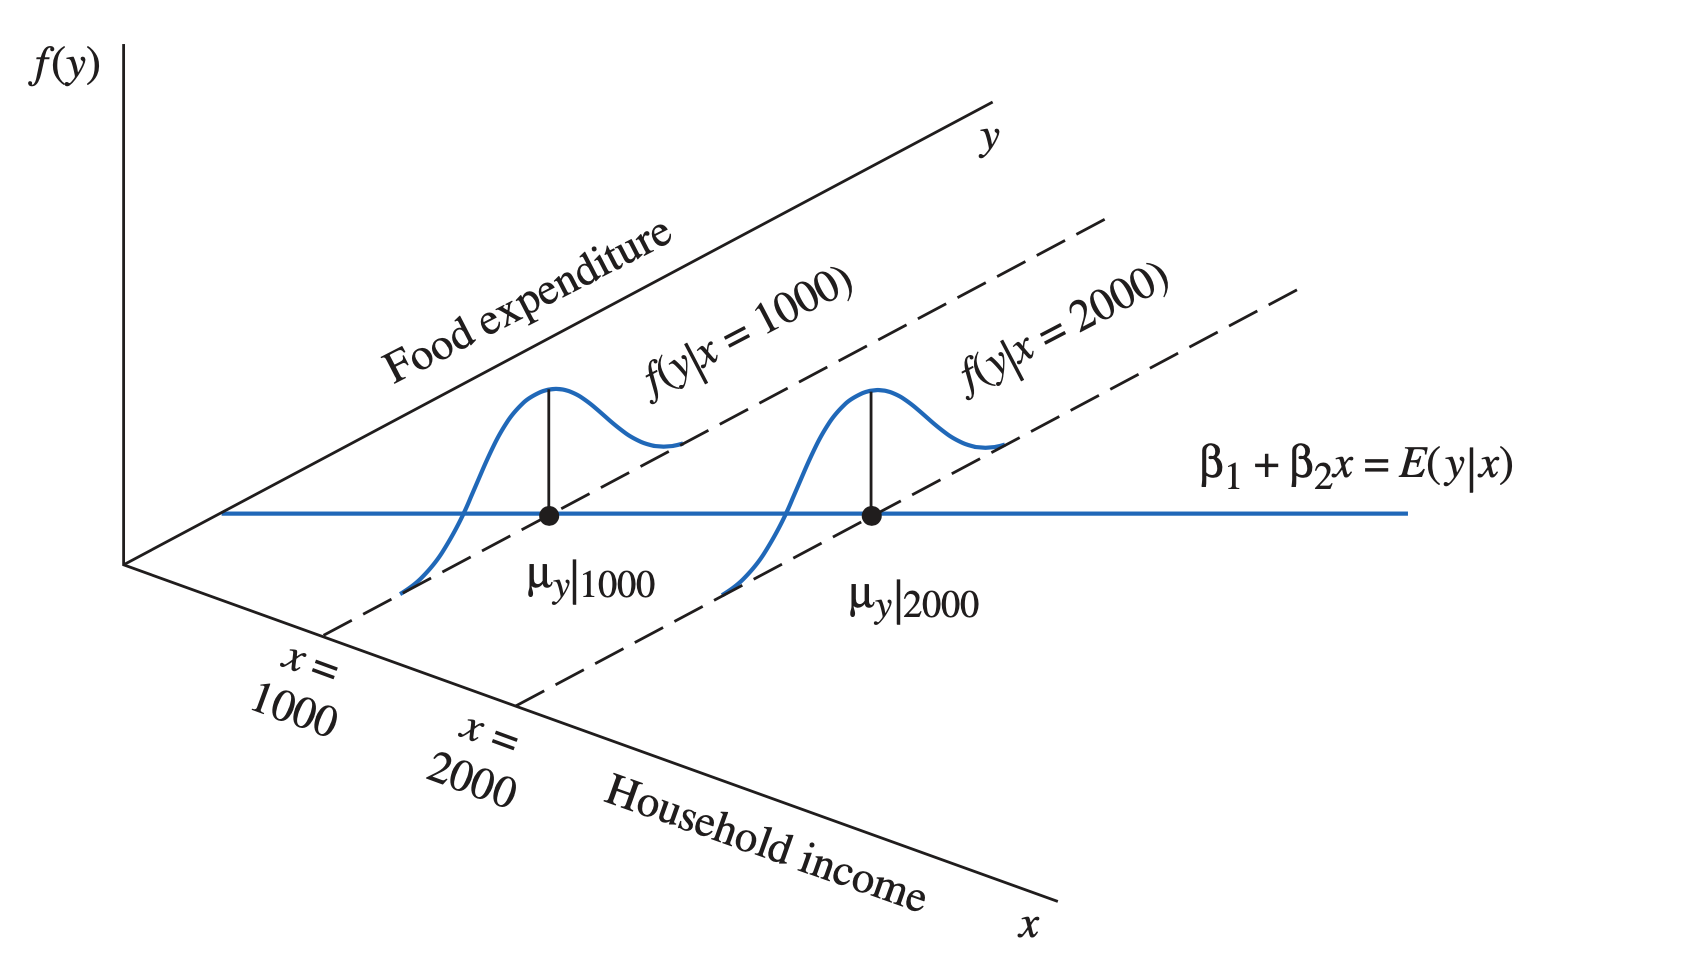
\includegraphics[width=0.5\linewidth]{food_homoskedasticity.png}
		\label{fig:food_homoskedasticity}
	\end{figure}}
	\onslide<2->

	Is this a reasonable assumption?
	\begin{itemize}
		\item<3-> Low income individuals don't have much choice on how much to spend on food 
		\item<4-> High income individuals may have high variance reflecting variance in taste
	\end{itemize}
	
\end{frame}
\begin{frame}{Inference: Heteroskedasticity} 
	\label{frame:h4}
	\ucla{Example 1}: Let \(Y\) be food expenditure and  \(X\) be household income and suppose we want to estimate the linear model.
	\[
	    Y = \ucla{\beta_0} + \ucla{\beta_1}X +\eps
	.\] 
	Homoskedasticity requires that the variance of food expenditures is the same for all levels of income. Instead we may expect the spread of food expenditure to depend on income
	\begin{figure}[htpb]
		\centering
		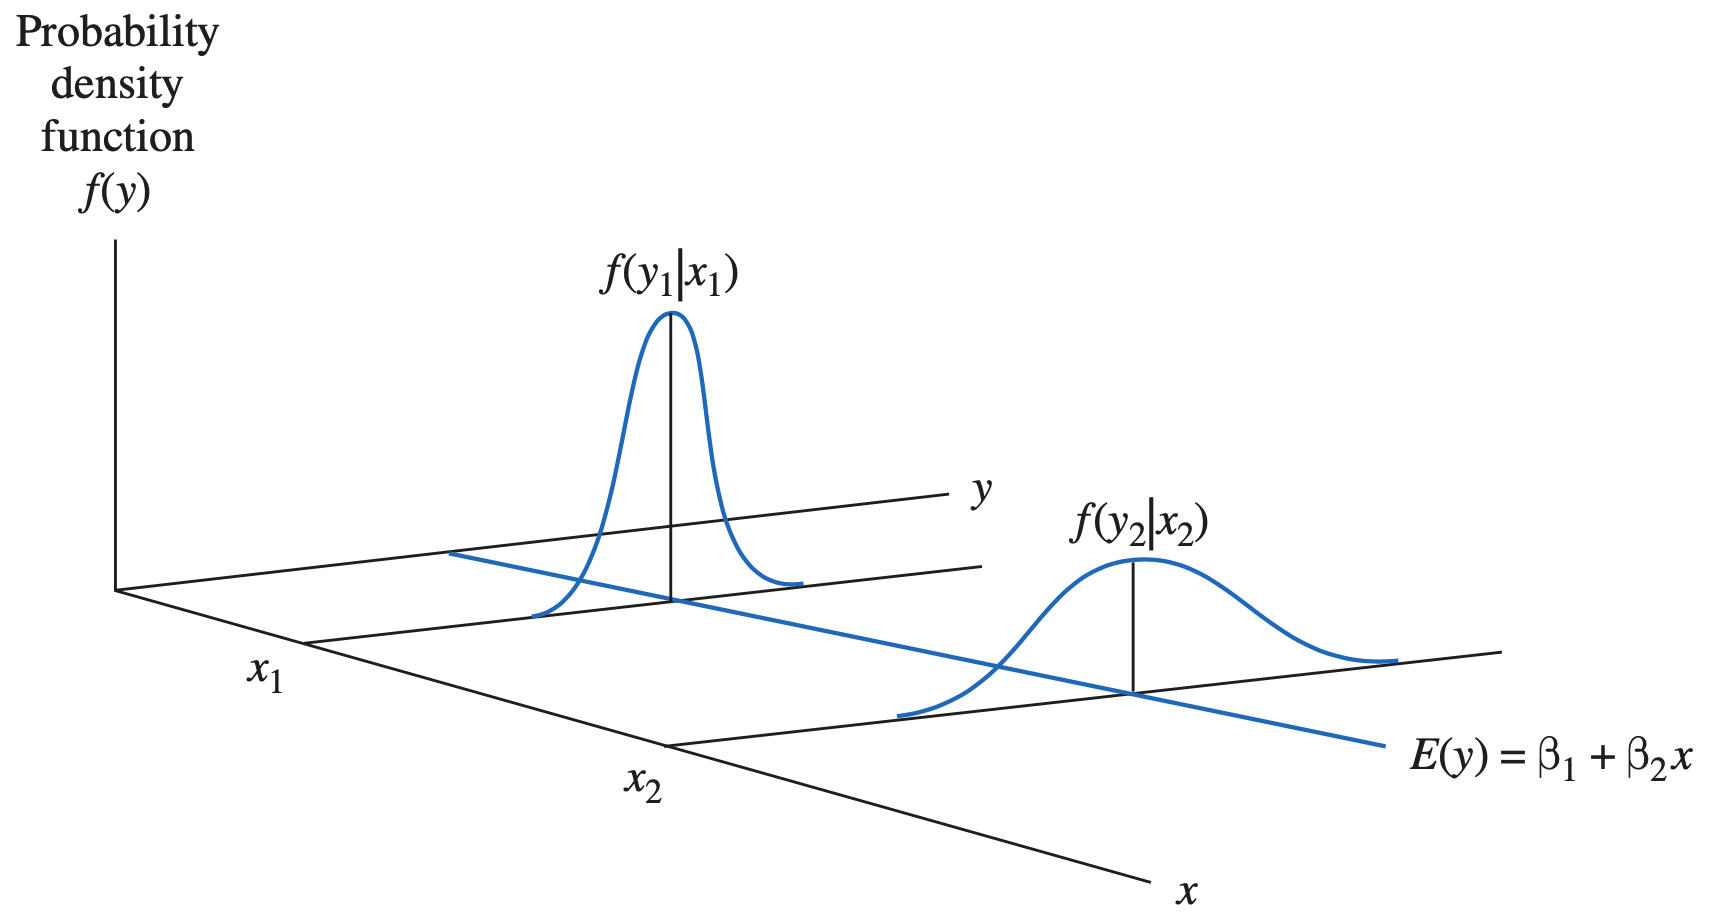
\includegraphics[width=0.5\linewidth]{food_heteroskedasticity.png}
	\end{figure}
\end{frame}
\begin{frame}{Inference: Heteroskedasticity} 
	\label{frame:h5}
	\ucla{Example 1}: Let \(Y\) be food expenditure and  \(X\) be household income and suppose we want to estimate the linear model.
	\[
	    Y = \ucla{\beta_0} + \ucla{\beta_1}X +\eps
	.\] 
	After estimating \(\ucla{\hat\beta_0}\) and \(\ucla{\hat\beta_1}\) we can check for heteroskedasticity by plotting the estimated residuals againt \(X\). \onslide<2-> In this case that looks like
	\begin{figure}[htpb]
		\centering
		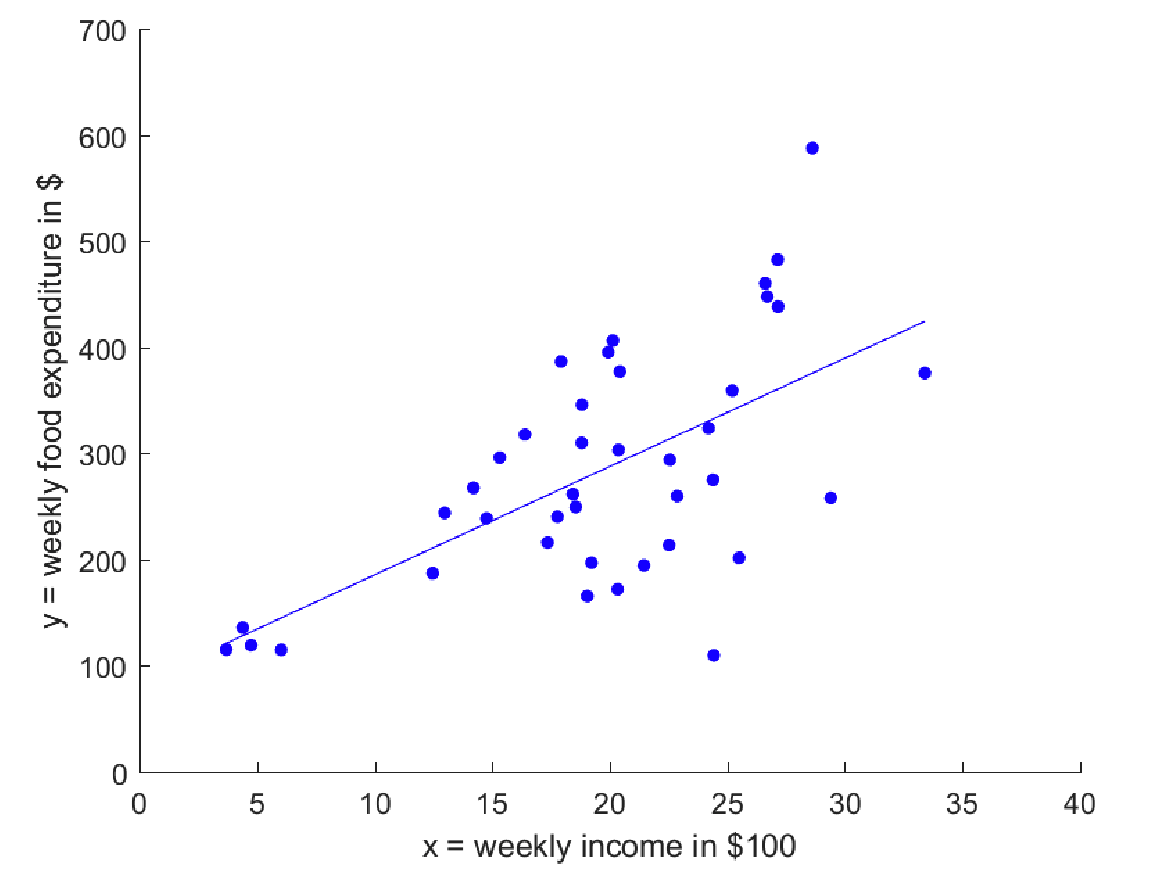
\includegraphics[width=0.45\linewidth]{food_scatter.png}
	\end{figure}
	\onslide<3->
	\begin{itemize}
		\item Residuals look more spread out for higher income levels, suggests homoskedasticity is violated
		\item Not a formal test (using \(\hat\eps\) instead of  \(\eps\)), but suggestive
	\end{itemize}
\end{frame}
\begin{frame}{Inference: Heteroskedasticity} 
	\label{frame:h6}
	\ucla{Example 2}: Let \(Y\) be wages and  \(X\) be years of education and consider the model 
	 \[
	    Y = \ucla{\beta_1} + \ucla{\beta_2}X + \eps
	.\] 
	In this context homoskedasticity requires that the variance in wages is the same for all levels of education.
	\only<2>{
	Is this a reasonable assumption?
	\begin{itemize}
		\item High school graduates may not have access to as many career paths
		\item College graduates can range from English PhDs to engineers at Google
	\end{itemize}}
	\only<3>{
	\begin{figure}[htpb]
		\centering
		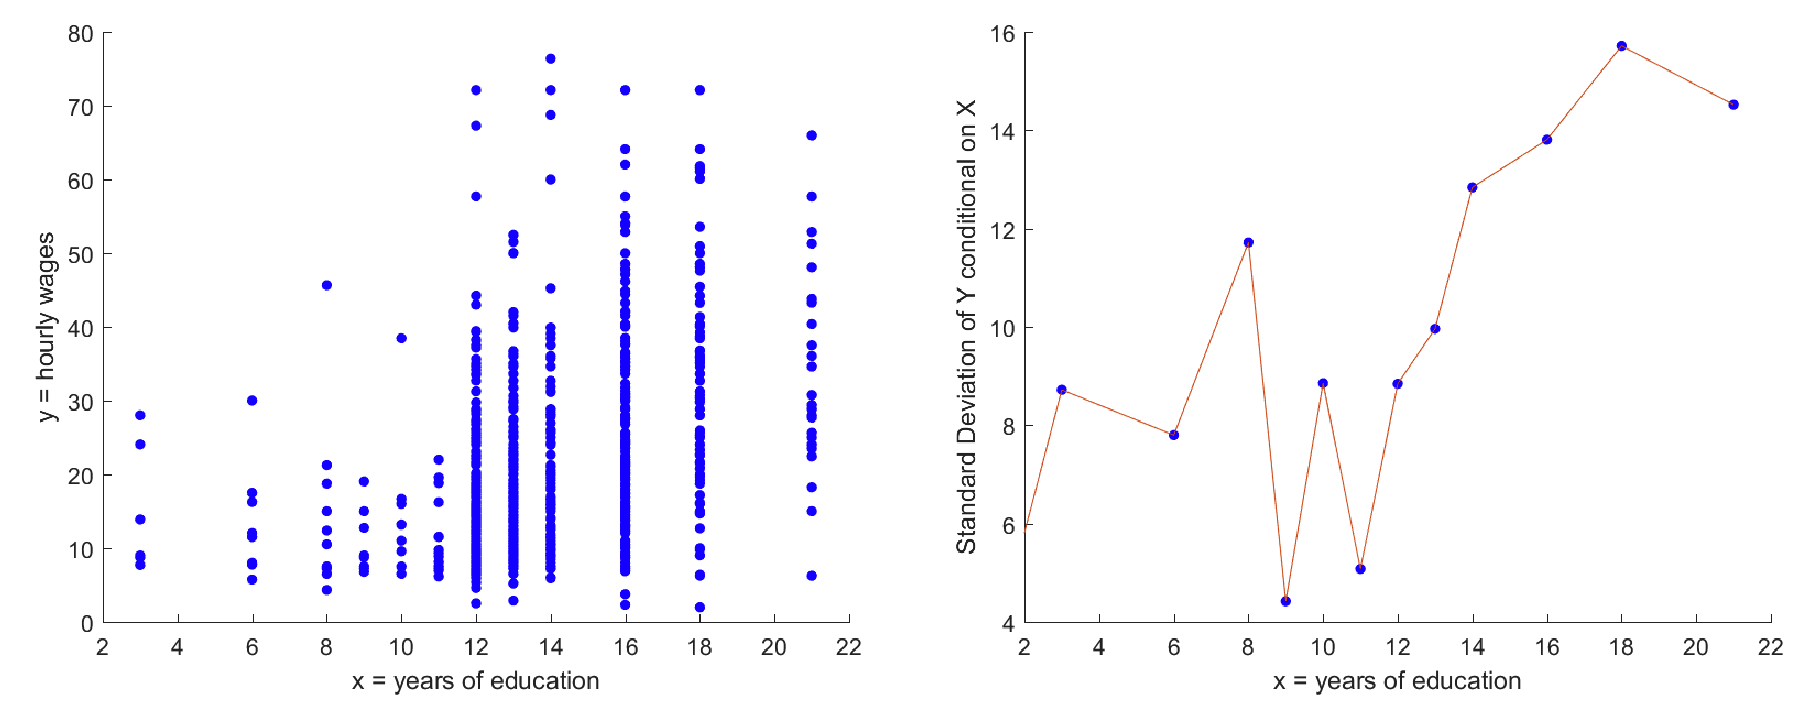
\includegraphics[width=0.8\linewidth]{edu_heteroskedasticity.png}
	\end{figure}
	\begin{itemize}
		\item Looking at the data we see that variance in wages increases increases after high school
	\end{itemize}
	}
\end{frame}
\begin{frame}{Heteroskedasticity: Questions}
	\centering
	\red{\Large Questions?}
\end{frame} 
%TODO: Add a homework question about binary X and heteroskedasticity in this context
%TODO: Maybe a good time to add a homework question about binary X and a linear model
\begin{frame}{Inference: Heteroskedasticity} 
	\label{frame:h7}
	So, suppose we look at our data and suspect homoskedasticity is violated. What do we do now?
	\begin{itemize}
		\item<1|only@1> Won't need to adjust our estimator 
	\end{itemize}
	\onslide<2->
	Recall that when were deriving the asymptotic distribution of our estimator \(\ucla{\hat\beta_1}\) (the approximate distribution for \(n\) large) we applied \red{law of large numbers} and found that approximately for large  \(n\):
	 \[
	 \sqrt{n}\left(\ucla{\hat\beta_1}-\ucla{\beta_1}\right) \approx \frac{\frac{1}{\sqrt{n}}\sum_{i=1}^n \eps_i(X_i-\mu_X)}{\sigma_X^2} 
	.\] 
	\onslide<3-> 
	We then applied the \red{central limit theorem} to \(\frac{1}{\sqrt{n}}\sum_{i=1}^n \eps_i(X_i-\mu_X)\): approximately for large \(n\),
	\[
		\frac{1}{\sqrt{n}}\sum_{i=1}^n \eps_i(X_i-\mu_X) \sim N\left(0,\Var(\eps(X-\mu_X))\right)
	.\] 
	\onslide<4->
	\begin{itemize}
		\item The only time we used homoskedasticity was to decompose \(\Var(\eps(X-\mu_X)) = \sigma_\eps^2\sigma_X^2\). This simplified estimation but is not necessary.
	\end{itemize}
\end{frame}
\begin{frame}{Inference: Heteroskedasticity} 
	\label{frame:h8}
	Without heteroskedasticity we can use the same logic as before without decomposing \(\Var(\eps(X-\mu_X)) = \sigma_\eps^2\sigma_X^2\) to get
	\[
		\sqrt{n}(\ucla{\hat\beta_1}-\ucla{\beta_1}) \sim N\left(0,\frac{\Var(\eps(X-\mu_X))}{(\sigma_X^2)^2}\right) \implies  \ucla{\hat\beta_1} \sim N\left(\ucla{\beta_1},\frac{\Var(\eps(X-\mu_X))}{n(\sigma_X^2)^2}\right)
	.\]
	\begin{itemize}
		\item<3-> Note that the variance still goes to \(0\) as  \(n\to\infty\) so that \( \ucla{\hat\beta_1}\to \ucla{\beta_1}\) as \(n\to\infty\).
		\item<4-> Asymptotic variance is different now however, and will require a different estimator.
		\item<5-> Using the wrong variance renders our inference useless as we will not be accurately computing objects like
			\[
				\Pr(|\ucla{\hat\beta_1}| > 5 | \ucla{\beta_1} = 0)
			.\] 
	\end{itemize}
\end{frame}
\begin{frame}{Inference: Heteroskedasticity} 
	\label{frame:h9}
	As mentioned above, all that needs to be done to relax homoskedasticity is find a way to estimate the asymptotic variance of \(\ucla{\hat\beta_1}\):
	\[
		\frac{\Var(\eps(X-\mu_X))}{(\sigma_X^2)^2} 
	.\] 
	\begin{itemize}
		\item<2-> Already know how to estimate \(\sigma_X^2\) 
		\item<3-> To estimate \(\Var(\eps(X-\mu_X))\) let  \(\hat W_i = \hat\eps_i(X_i - \bar X)\).
		\begin{itemize}
			\item<4-> Note that \(\frac{1}{n}\sum_{i=1}^n \hat\eps_i X_i = \bar X \frac{1}{n}\sum_{i=1}^n \hat\eps_i = 0\) by the first order conditions for \(\ucla{\hat\beta_1}\) and \( \ucla{\hat\beta_0}\), respectively. So \(\overline{\widehat W_i}  = \frac{1}{n}\sum_{i=1}^n \hat W_i = 0\).
			\item<5-> Can then estimate \(\Var(\eps(X -\mu_X))\) via
			 \[
				 \frac{1}{n}\sum_{i=1}^n \hat W_i^2
			.\]
		\item<6-> Since \(\hat\eps_i \to \eps_i\) and  \(\bar X \to \mu_X\),  \(\hat W_i \to \eps_i(X-\mu_X)\) and so we have a consistent estimator for \(\Var(\eps(X-\mu_X))\) by \red{law of large numbers}.
		\end{itemize}
	\end{itemize}
\end{frame}
\begin{frame}{Inference: Heteroskedasticity} 
	\label{frame:h10}
	To summarize under heteroskedasticity we have that (approximately for large \(n\))
	\[
		\sqrt{n}(\ucla{\hat\beta_1} - \ucla{\beta_1}) \sim N(0,\sigma_{\beta_1}^2) \implies \ucla{\hat\beta_1}\sim N(\ucla{\beta_1},\sigma_{\beta_1}^2/n)
	,\] 
	where \(\sigma_{\beta_1}^2 = \Var(\eps(X-\mu_X))/(\sigma_X^2)^2\).
	 \begin{itemize}
		 \item<2-> This is a different expression for \(\sigma_{\beta_1}^2\) than under homoskedasticity and involves a somewhat more complicated estimation procedure.
		 \item<3-> From now on we will generally assume heteroskedasticity. It is easy to let the computer handle estimation of the variance \(\sigma_{\beta_1}^2\) and the standard error \(\sigma_{\beta_1}/\sqrt{n}\).
		\item<4-> Formulas for variance of \(\ucla{\hat\beta_0}\) and the covariance between \( \ucla{\hat\beta_1}\) and \( \ucla{\hat\beta_0}\) will also be different. Again computer can handle these easily.
		\item<5-> Once the heteroskedastic-consistent variances/standard errors/covariances are computed inference and confidence intervals are computed the same as before.
	\end{itemize}
\end{frame}
\begin{frame}{Heteroskedasticity: Questions}
	\centering
	\red{\Large Questions?}
\end{frame} 

%TODO: Homework question, give some error plots and ask to detect heteroskedasticity
%TODO: Homework question; inference with heteroskedasticity
%TODO: If we have too much time cover white test 

\section{Evaluating our Model}
\begin{frame}{Evaluating our Model: Prediction} 
	\label{frame:g1}
	Let's switch tacks a bit and turn from inference to evaluating our model. Recall that we chose to model the relationship between  \(Y\) and  \(X\) by estimating the line of best fit between  \(Y\) and  \(X\):
	 \[
		 \ucla{\beta_0},\ucla{\beta_1} = \arg\min_{\tilde\beta_0,\tilde\beta_1}\E\left[(Y-\tilde\beta_0-\tilde\beta_1X)^2\right]
	.\]
	We then spent the next few days conducting inference on the parameters of interest \( \ucla{\beta_0}\) and \( \ucla{\beta_1}\).
	\onslide<2->

	Now, however, let's consider a different question. Is this even a good model? 
\end{frame}
\begin{frame}{Evaluating our Model: Prediction} 
	\label{frame:g2}
	When we are answering this question we are essentially interested in how our model does as a tool to \red{predict} \(Y\) using \(X\).
	\onslide<2->


	This is a somewhat different goal than in \red{inference} when we are interested in \green{interpreting} the parameters  \( \ucla{\beta_0}\) and \(\ucla{\beta_1}\) to learn about the underlying relationship between \(Y\) and  \(X\).
	\begin{itemize}
		\item Inference tends to be useful when thinking about policies to implement, want to know about average effects
	\end{itemize}
\end{frame}
\begin{frame}{Evaluating our Model: Prediction} 
	\label{frame:g3}
	Prediction can also be very useful though. Let's consider some examples.

	\only<2>{\ucla{Example}: How can Amazon do two day delivery?
	\begin{itemize}
		\item In order to deliver an item within two days, an item has to be in stock in a warehouse nearby
		\item If too many people buy the item at once in a certain area the warehouse will run out of stock
		\item Amazon has to be able to accurately \red{forecast/predict} demand in certain areas.
	\end{itemize}}
	\only<3>{\ucla{Example}: How much power should the energy grid generate?
	\begin{itemize}
		\item Energy grid must have enough supply to meet demand
		\item But it is costly and takes time to adjust production levels
		\item Energy suppliers must have good forecasts of demand
	\end{itemize}}
	\onslide<4->{\ucla{Example}: How much should a pension fund keep in liquid funds?
	\begin{itemize}
		\item Fund must be able to pay all it's obligations
		\item Some portion of funds are invested and returns are random. People also retire/die at random times.
		\item Pension fund must forecast both obligations and returns.
	\end{itemize}}	
	\onslide<5->
	Note that in these examples we are not per-se interested in interpreting the parameters of our linear regression model. We are just interested in using our linear regression model to predict \(Y\) using  \(X\).
\end{frame}
\begin{frame}{Evaluating our Model: Prediction} 
	\label{frame:f4}
	Suppose we had no information on \(X\). What is the best we can do in terms of predicting  \(Y\)?
	\begin{itemize}
		\item If we just have information on income and we are given a random name, what should we predict their income to be?
	\end{itemize}
	\onslide<2->

	Since we have no additional information, we will make the same prediction for all new observations. Want to choose a value \(a*\) that minimizes 
	\[
		a^* = \arg\min_a\E[(Y-a)^2]
	.\] 
	That is \(a^*\) is  ``closest'' to \(Y\) on average.
\end{frame}
\begin{frame}{Evaluating our Model: Prediction} 
	\label{frame:f5}
	Taking first order conditions, we see that \(a^*\) solves
	\[
		-2\E[(Y-a^*)] = 0 \implies a^* = \E[Y]
	.\] 
	\onslide<2-> 
	The best predictor of \(Y\) with no additional information is just  \(\E[Y]\)! 
	\begin{itemize}
		\item This is intuitive enough
	\end{itemize}
\end{frame}
\begin{frame}{Evaluating our Model: Prediction} 
	\label{frame:f6}
	Now that we have information on \(X\) we have tried to use this information to predict \(Y\) by estimating a line of best fit (linear model) between  \(Y\) and  \(X\):
	 \[
		 \ucla{\beta_0},\ucla{\beta_1} = \arg\min_{\tilde\beta_0,\tilde\beta_1}\E\left[(Y-\tilde\beta_0-\tilde\beta_1X)^2\right]
	.\]
	\onslide<2->
	\red{Question}: How much better is this linear model at predicting \(Y\) than just using  \(\E[Y]\)?
	\begin{itemize}
		\item<3-> Obviously cannot evaluate this directly since we don't know \( \ucla{\beta_0},\ucla{\beta_1}\) and \(\E[Y]\)
		\item<4-> Instead we will see how much closer \(\hat Y_i = \ucla{\hat\beta_1} + \ucla{\hat\beta_1} X_i\) is to \(Y_i\) on average than \(\bar Y\).
	\end{itemize}
\end{frame}
\begin{frame}{Evaluating our Model: \(R^2\) and Goodness of Fit} 
	\label{frame:f7}
	Let's recall the following equalities implied by the first order conditions of our estimating equations
	\[
		\ucla{\hat\beta_0}, \ucla{\hat\beta_1} = \arg\min_{b_0,b_1}\frac{1}{n}\sum_{i=1}^n (Y_i-b_0-b_1X_i)^2
	.\]
	\onslide<2->
	From the first order condition for \(\ucla{\hat\beta_0}\):
	\[
		\frac{1}{n}\sum_{i=1}^n (Y_i - \ucla{\hat\beta_0}-\ucla{\hat\beta_1}X_i)^2 =  \frac{1}{n}\sum_{i=1}^n \hat\eps_i = 0
	.\] 
	From the first order condition for \(\ucla{\hat\beta_1}\):
	\[
		\frac{1}{n}\sum_{i=1}^n  (Y_i - \ucla{\hat\beta_0}-\ucla{\hat\beta_1}X_i)X_i = \frac{1}{n}\sum_{i=1}^n \hat\eps_i X_i = 0
	.\]
	
\end{frame}
\begin{frame}{Evaluating our Model: \(R^2\) and Goodness of Fit} 
	\label{frame:f8}	
	Recall that, by definition of \(\hat\eps_i = Y_i - \ucla{\hat\beta_0} -\ucla{\hat\beta_1} X_i\)
	\[
	    Y_i = \ucla{\hat\beta_0} + \ucla{\hat\beta_1}X_i + \hat\eps_i  = \hat Y_i + \hat\eps_i
	.\] 	
	and that after solving for \( \ucla{\hat\beta_0}\) we get
	\[
	    \ucla{\hat\beta_0} = \bar Y - \ucla{\hat\beta_1}\bar X \implies \bar Y = \ucla{\hat\beta_0} + \ucla{\hat\beta_1}\bar X
	.\] 	
	\onslide<2->
	Using these we get that
	\begin{align*}
		Y_i - \bar Y &= (\hat Y_i - \bar Y)  + \hat\eps_i \\
					 &= \ucla{\hat\beta_1}(X_i - \bar X) + \hat\eps_i
	\end{align*}
\end{frame}
\begin{frame}{Evaluating our Model: \(R^2\) and Goodness of Fit} 
	\label{frame:f9}
	Now let's use these and decompose the sum:
	\begin{align*}
		\overbrace{\sum_{i=1}^n (Y_i - \bar Y)^2}^{\text{Total variance in \(Y\)}} &= \sum_{i=1}^n (\hat Y_i - \bar Y)^2 + \frac{1}{n}\sum_{i=1}^n (Y_i - \bar Y)\eps_i +  \frac{1}{n}\sum_{i=1}^n \hat\eps_i^2 \\
		\onslide<2->{
		&= \frac{1}{n}\sum_{i=1}^n (\hat Y_i - \bar Y)^2 + \ucla{\hat\beta_1}\overbrace{\frac{1}{n}\sum_{i=1}^n (X_i - \bar X)\hat\eps_i}^{=0\text{ by FOCs}} + \frac{1}{n}\sum_{i=1}^n \hat\eps_i^2 \\}
		\onslide<3->{
		&= \underbrace{\frac{1}{n}\sum_{i=1}^n  (\hat Y_i - \bar Y)^2}_{\text{Explained by model with \(X\)}} + \underbrace{\frac{1}{n}\sum_{i=1}^n \hat\eps_i^2}_{\text{unexplained by model}}}
	\end{align*}	
\end{frame}
\begin{frame}{Evaluating our Model: \(R^2\) and Goodness of Fit} 
	\label{frame:f10}
	Often we multiply both sides of the last equation by \(n\) and label the resulting components:
	\[
		\sum_{i=1}^n (Y_i - \bar Y)^2 = \sum_{i=1}^n  (\hat Y_i - \bar Y)^2 +\sum_{i=1}^n \hat\eps_i^2
	.\] 
	\begin{enumerate}
		\item<1-> \ucla{\(\sum_{i=1}^n (Y_i - \bar Y)^2\)}: \red{SST (Total Sum Of Squares)}
		\begin{itemize}
			\item Captures how much total variation there is in \(Y\).
			\item Can think of this as the sum of squared errors from just using \(\bar Y\) to predict  \(Y\).
			\item Note that this is just the sample variance of \(Y\) multiplied by \(n\)
		\end{itemize}
		\item<2-> \ucla{\(\sum_{i=1}^n (\hat Y_i - \bar Y)^2\)}: \red{SSR (Sum of Squares due to Regression)}
		\begin{itemize}
			\item Captures variation that can be attributed to variation in our predictions
			\item This is the sample variance of \(\hat Y_i\) multiplied by \(n\) 
		\end{itemize}
		\item<3-> \ucla{\(\sum_{i=1}^n \hat\eps_i^2\)}: \red{SSE (Sum of Squared Errors)}
		\begin{itemize}
			\item Variation that is ``left over'' after using the linear model
			\item Note that this is just  \(\hat\sigma_\eps^2\) times  \(n\)
		\end{itemize}
	\end{enumerate}
\end{frame}
\begin{frame}{Evaluating our Model: \(R^2\) and Goodness of Fit} 
	\label{frame:f11}
	Using the decomposition
	\[
		\underbrace{\sum_{i=1}^n (Y_i - \bar Y)^2}_{\text{SST}} = \underbrace{\sum_{i=1}^n  (\hat Y_i - \bar Y)^2}_{\text{SSR}} +\underbrace{\sum_{i=1}^n \hat\eps_i^2}_{\text{SSE}}
	.\] 
	we define the coefficient of determination, \(R^2\), as
	\[
		R^2 = \frac{\text{SSR}}{\text{SST}} = 1 - \frac{\text{SSE}}{\text{SST}}  
	.\]
	\onslide<2->
	\begin{itemize}
		\item<2-> Intuitively \(R^2\) reports what proportion of the total variance in  \(Y\) can be explained by our linear model with  \(X\). 
		\item<3-> \(R^2\) is generally reported when running a regression by almost any statistical software.
	\end{itemize}
\end{frame}
\begin{frame}{Evaluating our Model: \(R^2\) and Goodness of Fit} 
	\label{frame:f12}
	Let's see how this looks with an example from two different datasets
	\begin{figure}[htpb]
		\centering
		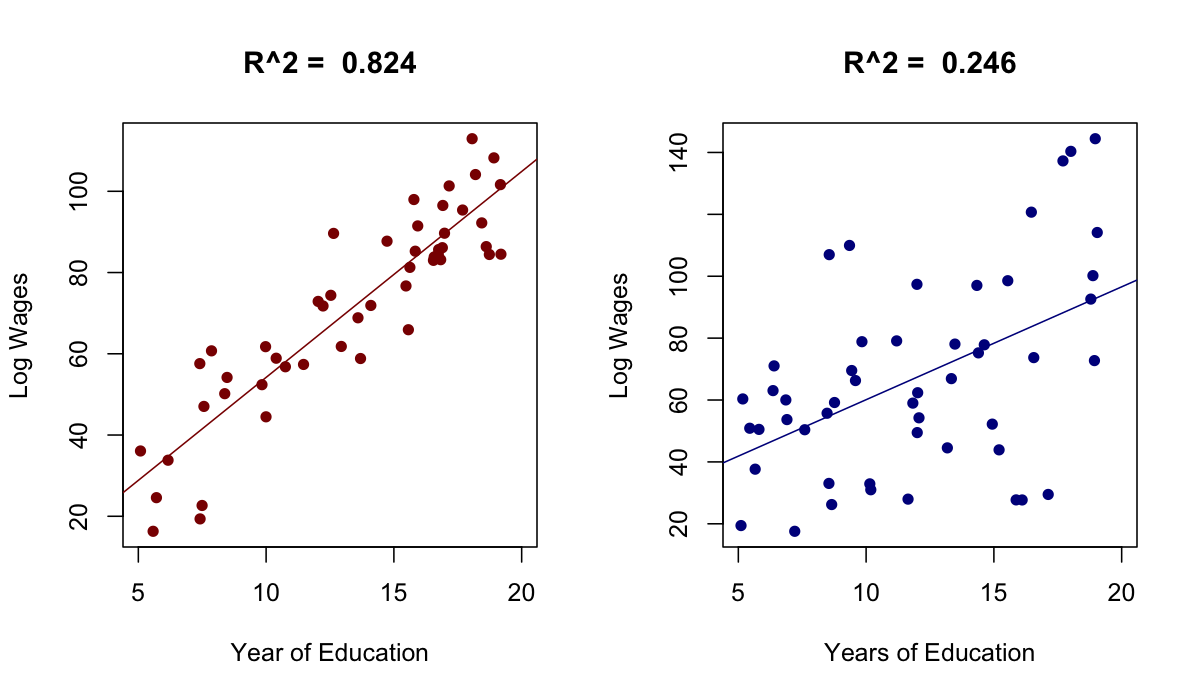
\includegraphics[width=0.8\linewidth]{R2.png}
	\end{figure}
	\begin{itemize}
		\item<2-> In which dataset does the regression line look closer to the data?
		\item<3-> Does homoskedasticity look to be violated here?
	\end{itemize}
\end{frame}

\section{Modeling Choices}%
%NOTE: Stability under linear transformations, nonlinear transformations/elasticity
\begin{frame}{Modeling Choices: Transforming our Data} 
	\label{frame:m1}
	Suppose we fit our linear model and find a low \(R^2\). There are two main reasons this could be happening.
	\begin{enumerate}
		\item<1-> Knowing \(X\) simply does not give us much information about  \(Y\)
		 \begin{itemize}
			\item<2-> For example, suppose we were trying to predict log wages, \(Y\), using a persons favorite color,  \(X\).
		\end{itemize}
		\item<3-> The true relationship between \(X\) and  \(Y\) is non-linear and we are trying to fit a linear model.
	\end{enumerate}
	\onslide<4->
	The first problem we can't do much to address, other than trying to collect more right hand side variables. The second problem however we can try and address by \ucla{transforming our data}.
\end{frame}
\begin{frame}{Modeling Choices: Transforming our Data} 
	\label{frame:m2}
	Let's see an example of this. Suppose we collect our data and it looks like below
	\begin{figure}[htpb]
		\centering
		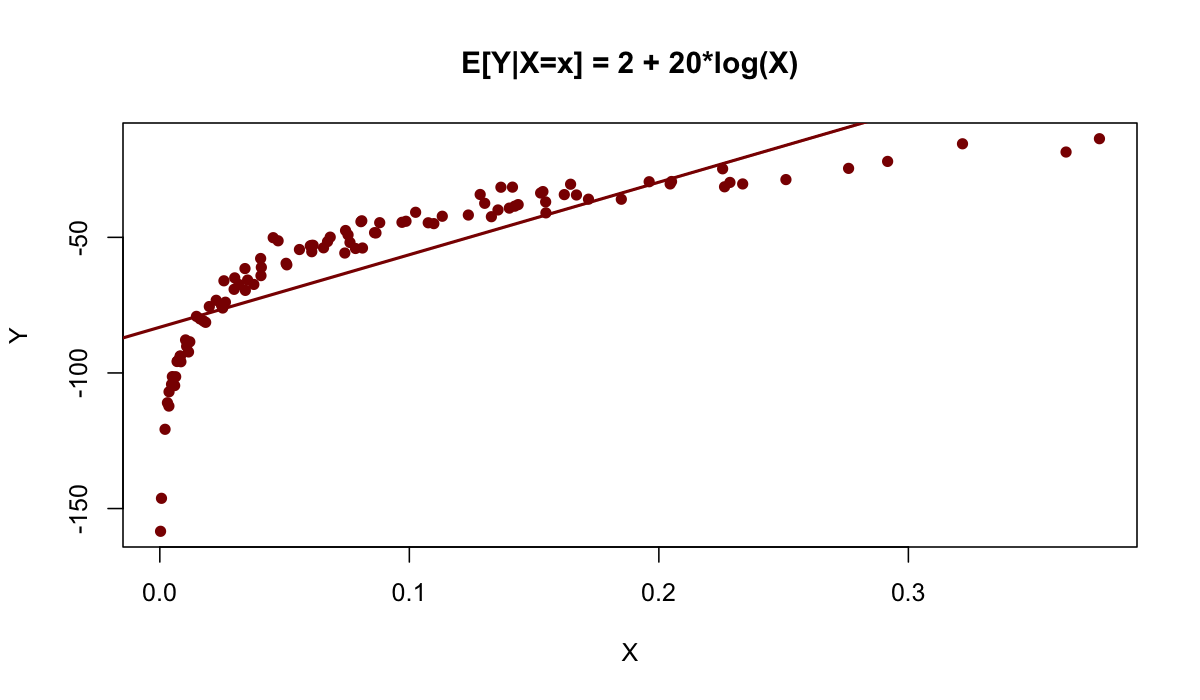
\includegraphics[width=0.8\linewidth]{nonlinear1.png}
	\end{figure}
	\onslide<2-> 
	The relationship between \(X\) and  \(Y\) is clearly non-linear, but we are trying to fit a line through it. This hurts our model preformance.
\end{frame}
\begin{frame}{Modeling Choices: Transforming our Data} 
	\label{frame:m3}
	Other reasons that we may think that the relationship between \(Y\) and  \(X\) is non-linear
	\begin{itemize}
		\item \(Y\) is bounded and \(X\) has a large support.
		\begin{itemize}
			\item<3-> For example, suppose \(Y\in\{0,1\}\) denotes treatment uptake and \(X\) denotes income.
			\item<4-> A linear model of the form \( \ucla{\beta_0} + \ucla{\beta_1}\cdot X\) would give \(\hat Y > 1\) for a sufficiently large value of  \(X\).
		\end{itemize}
		\item<5-> We believe that the derivative of \(Y\) with respect to  \(X\) is not constant.
		 \begin{itemize}
			\item<6-> Suppose \(Y\) is amount spent on groceries and \(X\) is income.
			\item<7-> We expect that as income rises people may start shopping at Whole Foods or spending more on nicer ingredients.
			\item<8-> But this will probably level off for high levels of income. A linear model imposes that \(\frac{d}{dx}\hat{Y}(x) = \frac{d}{dx}(\ucla{\beta_0} + \ucla{\beta_1}x) = \ucla{\beta_1}\) for all \(x\).
		\end{itemize}
	\end{itemize}
\end{frame}
\begin{frame}{Modeling Choices: Transforing our Data} 
	\label{frame:m4}
	So, given that we believe the relationship between \(Y\) and  \(X\) to be nonlinear, what can we do about this?
	\onslide<2->

	Before we move on to something fancier, let's try just transforming our data and running a linear regression:
	\[
		f(Y) = \ucla{\beta_0} + \ucla{\beta_1}g(X) + \eps
	.\]

	\onslide<3->
	Common functions to be used here are \(\ln(z)\),  \( \sqrt{z}\), and various polynomials; \(z^2, z^3\), etc.
\end{frame}
\begin{frame}{Modeling Choices: Transforming our Data} 
	\label{frame:m5}
	Let's return to our data from before and see how this would work. 
	\only<1>{
	\begin{figure}[htpb]
		\centering
		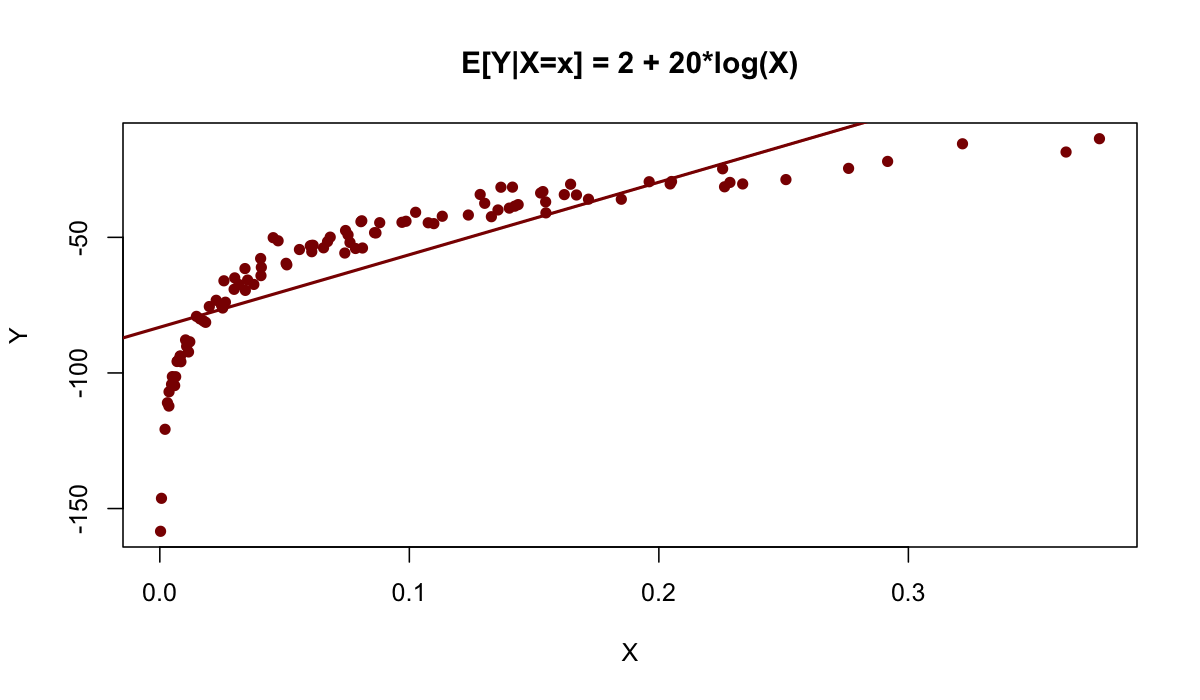
\includegraphics[width=0.75\linewidth]{nonlinear1.png}
	\end{figure}
	}
	\only<2>{
	\begin{figure}[htpb]
		\centering
		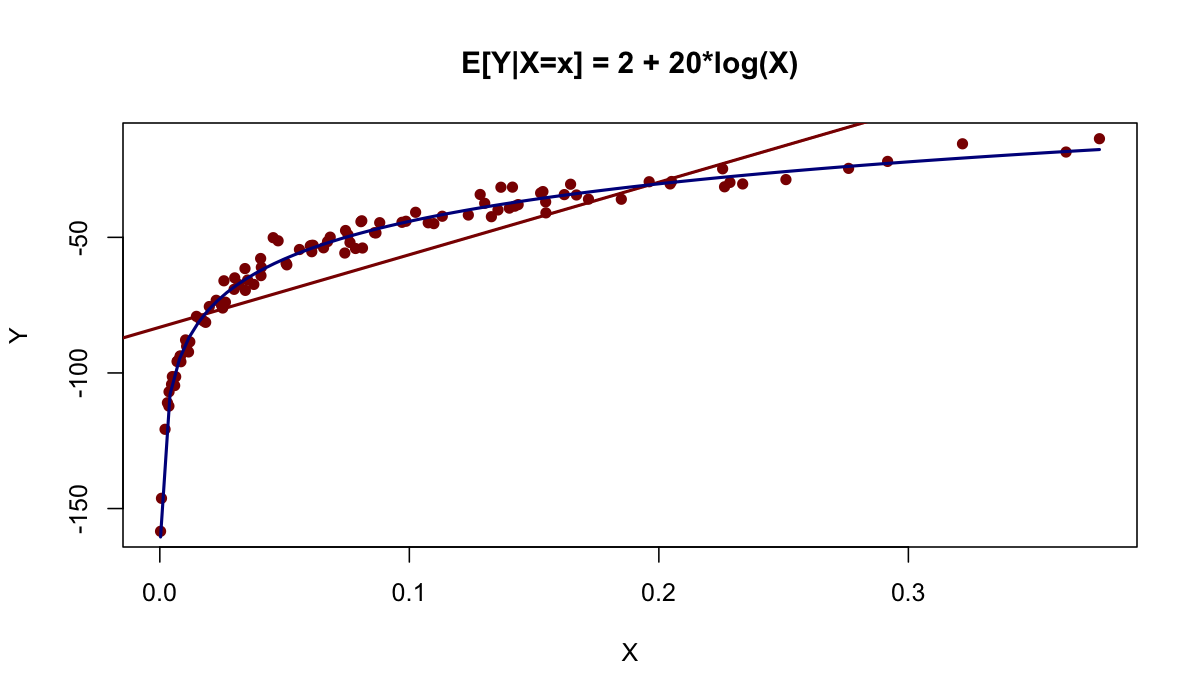
\includegraphics[width=0.75\linewidth]{nonlinear2.png}
	\end{figure}
	}
	Instead of fitting the model \(Y = \ucla{\beta_0} + \ucla{\beta_1}X +\eps\) let's try fitting the model \(Y = \ucla{\beta_0} + \ucla{\beta_1}\ln(X) + \eps\)
	\begin{itemize}
		\item<1|only@1> How is this done? Choose our estimates
			\[
				\ucla{\hat\beta_0},\ucla{\hat\beta_1} = \arg\min_{b_0,b_1} \frac{1}{n}\sum_{i=1}^n \left(Y_i - b_0 - b_1\cdot\ln(X_i)\right)^2
			.\] 
		\item<2|only@2> We can see that the blue regression line is much closer to the data on average (\(R^2 = 0.988\) vs  \(R^2 = 0.6536\))
	\end{itemize}	
\end{frame}
\begin{frame}{Modeling Choices: Transforming our Data} 
	\label{frame:m6}
	Let's see another example. Suppose our data looks like the below.
	\only<1>{
	\begin{figure}[htpb]
		\centering
		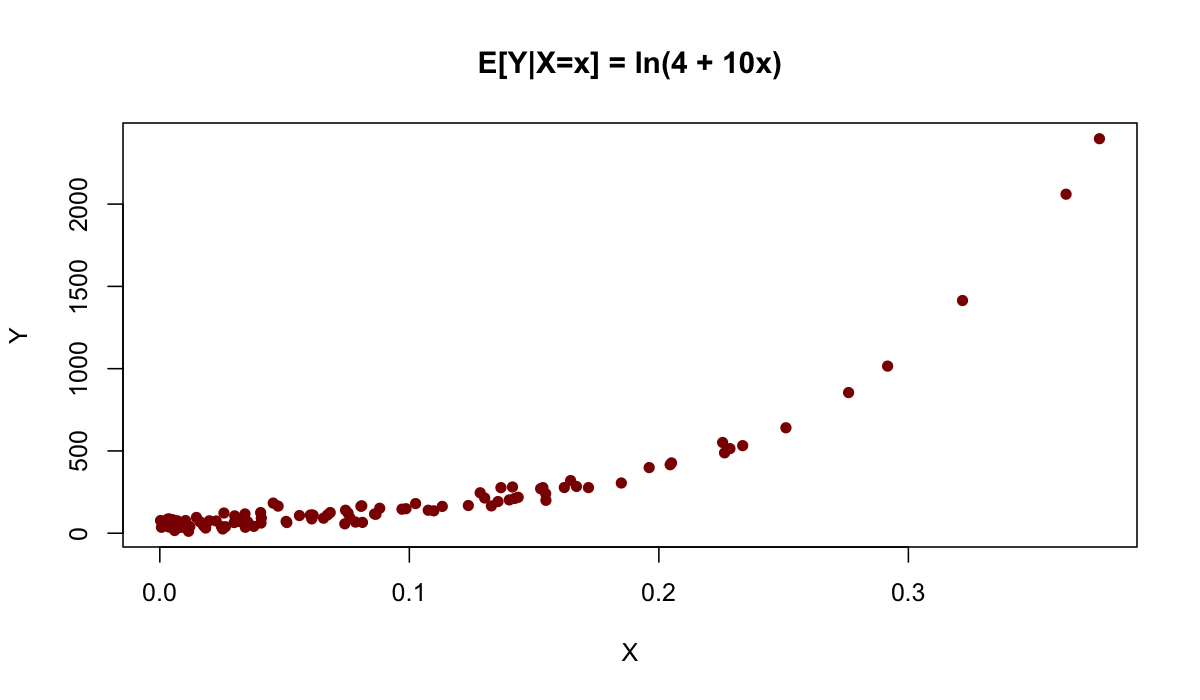
\includegraphics[width=0.8\linewidth]{nonlinearPoints2.png}
	\end{figure}
	First, let's try fitting a non-transformed linear regression: \(Y = \ucla{\beta_0} + \ucla{\beta_1}X+\eps\)}
	\only<2>{
	\begin{figure}[htpb]
		\centering
		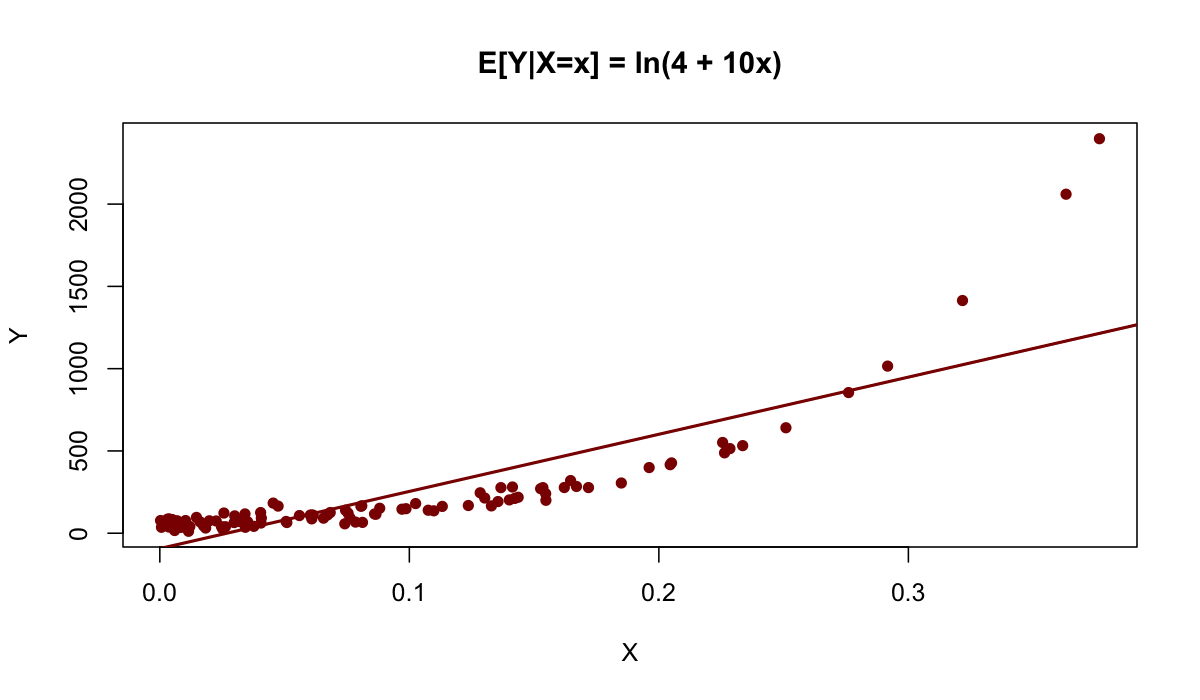
\includegraphics[width=0.8\linewidth]{nonlinear3.png}
	\end{figure}
	We see that this line does not appear to be fitting the data so well (\(R^2 = 0.692\)). Because \(Y\) apears to grow exponentially with  \(X\), we may want to try transforming  \(Y\).}
	\only<3>{
	\begin{figure}[htpb]
		\centering
		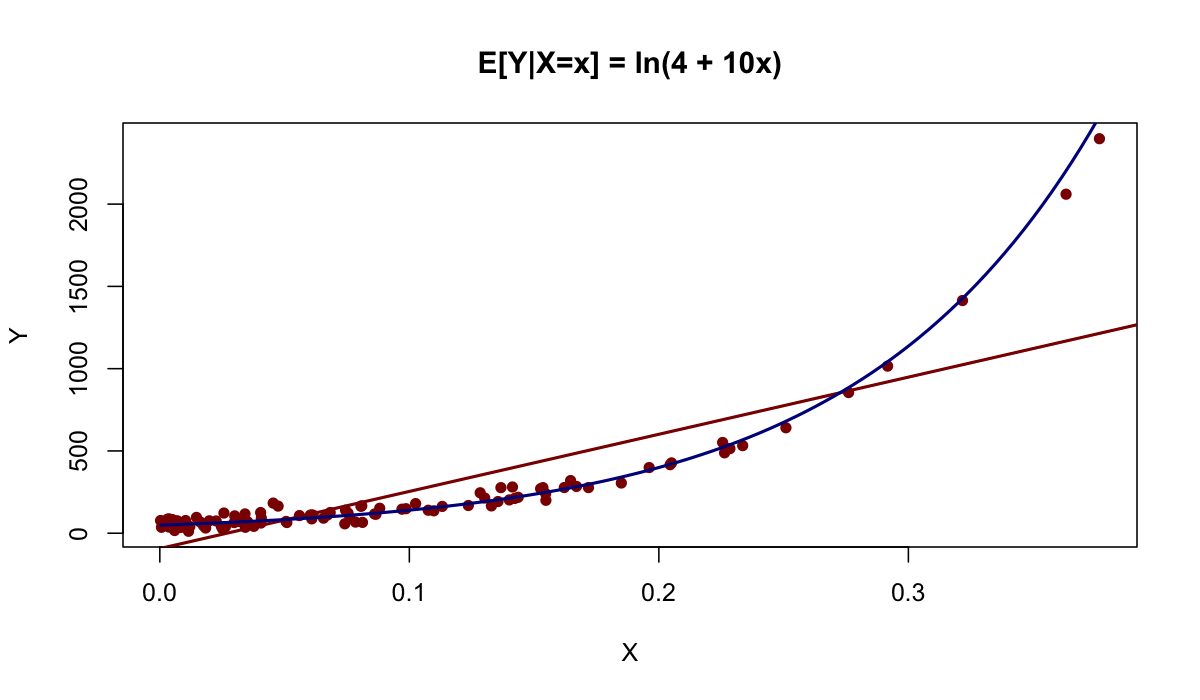
\includegraphics[width=0.8\linewidth]{nonlinear4.png}
	\end{figure}
	The blue curve is our estimate of the model \(\ln(Y) = \ucla{\beta_0} + \ucla{\beta_1}X + \eps\). This fits the data much better and gives \(R^2 = 0.8553\). We estimate the parameters via
	\[
		\ucla{\hat\beta_0},\ucla{\hat\beta_1} = \arg\min_{b_0,b_1}\frac{1}{n}\sum_{i=1}^n (\ln(Y_i) - b_0 - b_1X_i)^2
	.\] 
	}	
\end{frame}
\begin{frame}{Modeling Choices: Transforming our Data} 
	\label{frame:m7}
	In all of the above, notice that from an estimation and inference perspective, nothing much has changed. We can estimate our parameters and conduct inference just as before, but while treating our data as \(\{f(Y_i),g(X_i)\}\) as opposed to \(\{Y_i,X_i\}\).
\end{frame}
\begin{frame}{Modeling Choices: Transforming our Data} 
	\label{frame:m8}
	Let's see an example of this. Suppose that we want to estimate the following model:
	\[
		\ln(Y) = \ucla{\beta_0} + \ucla{\beta_1}\cdot \ln(X) + \eps
	.\] 
	\onslide<2->
	Using our data \(\{Y_i,X_i\}\) we estimate \( \ucla{\hat\beta_0},\ucla{\hat\beta_1}\) via
	\[
		\ucla{\hat\beta_0},\ucla{\hat\beta_1} = \arg\min_{b_0,b_1}\frac{1}{n}\sum_{i=1}^n (\ln(Y_i) - b_0 - b_1X_i)^2
	.\]
	we find that, with \(n = 49\), \(\ucla{\hat\beta_1} = 0.5\), \(\sigma_{\ln(X)}^2 = \frac{1}{n}\sum_{i=1}^n (\ln(X_i) - \overline{\ln(X)})^2 = 4\) and \(\hat \sigma_\eps^2 = \frac{1}{n}\sum_{i=1}^n (\ln(Y_i) - \ucla{\hat\beta_0} - \ucla{\hat\beta_1}\ln(X_i))^2 = 4\). 

\end{frame}
\begin{frame}{Modeling Choices: Transforming our Data} 
	\label{frame:m9}
	Assuming homoskedasticity, let's use this information to construct a \(95\%\) confidence interval for  \(\ucla{\hat\beta_1}\).
	\onslide<2->

	We use the same formula from before to calculate \(\hat\sigma_{\beta_1}^2 = \frac{\hat\sigma_\eps^2}{\hat\sigma_{\ln(X)}^2} =\frac{4}{4}=  1\).
	
	Then, using \(z_{0.975} = 1.96\), a \(95\%\) confidence interval is contructed
	\[
		\ucla{\hat\beta_1} \pm 1.96\frac{\hat\sigma_{\beta_1}}{\sqrt{n}} = 0.5 \pm 1.96\frac{1}{7}  = [0.22,0.78]  
	.\]
	\onslide<3->
	\begin{itemize}
		\item<4-> Notice that everything is the same as before
		\item<5-> Using this, would we reject \(\green{H_0}:\ucla{\beta_1} \leq 0\) against \(\red{H_1}:\ucla{\beta_1} > 0\) at level \(\alpha = 0.5\)?
		\begin{itemize}
			\item<6-> Recall that we would reject \(\green{H_0}:\ucla{\beta_1}= 0\) against \(\red{H_1}:\ucla{\beta_1} \neq 0\) at level \(\alpha = 0.5\).
		\end{itemize}
	\end{itemize}	
\end{frame}
\begin{frame}{Transforming our Data: Questions}
	\centering
	\red{\Large Questions?}
\end{frame} 

\begin{frame}{Modeling Choices: Transforming our Data} 
	\label{frame:m10}
	What changes, however, is our interpretation of our parameters. Before we interpreted:
	\begin{itemize}
		\item \(\ucla{\beta_0}\): Expected value of \(Y\) when  \(X = 0\).
		\item \(\ucla{\beta_1}\): Expected change in \(Y\) when  \(X\) increases by one unit
	\end{itemize}
	\onslide<2->
	\vspace{0.3cm}

	In the model \(f(Y) = \ucla{\beta_0} + \ucla{\beta_1}g(X) + \eps\), we have the following interpretations of \( \ucla{\beta_0}\) and \(\ucla{\beta_1}\).
	\begin{itemize}
		\item \(\ucla{\beta_0}\): Expected value of \(f(Y)\) when \(g(X) = 0\) 
		\item \(\ucla{\beta_1}g'(x)\): Expected change in \(f(Y)\) at \(X=x\) when \(X\) increases by one unit.
	\end{itemize}
\end{frame}
\begin{frame}{Modeling Choices: Transforming our Data} 
	\label{frame:m11}
	\ucla{Example}: Suppose \(X\) represents the square footage of a house and  \(Y\) represents is final sales price (in tens of thousands of dollars). We estimate the following model
	 \[
	    Y = \ucla{\beta_0} + \ucla{\beta_1}X^2 + \eps
	\] 
	and find that \(\ucla{\hat\beta_0} = 50\) and \(\ucla{\hat\beta_1} = 2\).
	\onslide<2->

	\red{How do we interpret these parameter estimates?}
	\begin{itemize}
		\item \(\ucla{\hat\beta_0} = 50\): The expected sales price of an empty lot (\(X^2 = 0 \iff X=0\)) is \$50,000.
		\item<3-> \( \ucla{\hat\beta_1} = 2\): Taking derivatives gives that \(\frac{d}{dx}\hat Y = 2\ucla{\hat\beta_1}X\). We expect that a one square foot increase in home size at square footage \(x\) will be associated with a \$40,000\(\cdot\)x increase in sales price.
	\end{itemize}
\end{frame}
\begin{frame}{Modeling Choices: Transforming our Data} 
	\label{frame:m12}
	A useful approximation that we use here is that a one unit increase in \(\ln(Z)\) is about a  \(100\%\) increase in \(Z\) and vice versa, a \(1\%\) increase in  \(Z\) is associated with a  \(1/100\) unit increase in \(\ln(Z)\). 

	This is useful for interpreting the parameters of various models.
	\begin{itemize}
		\item Suppose we model \(Y = \ucla{\beta_0} + \ucla{\beta_1}\ln(X) + \eps \implies\) a \(1\%\) increase in  \(X\) is associated with a  \(\ucla{\beta_1}/100\) unit change in \(Y\).
		\item<2-> Suppose we model \(\ln(Y) = \ucla{\beta_0} + \ucla{\beta_1}X + \eps \implies\) a \(1\) unit increase in  \(X\) is associated with  \(100\cdot\ucla{\beta_1}\%\) increase in \(Y\)
		\item<3-> Suppose we model \(\ln(Y) = \ucla{\beta_0} + \ucla{\beta_1}\ln(X) + \eps \implies\) a \(1\%\) increase is associated with a  \(\ucla{\beta_1}\%\) increase in \(Y\).
	\end{itemize}
\end{frame}
\begin{frame}{Transforming our Data: Questions}
	\centering
	\red{\Large Questions?}
\end{frame} 
\begin{frame}{Modeling Choices: Linear Transformations} 
	\label{frame:m13}
	
\end{frame}


%TODO: Assign linear transfomrations as a homework problem

\end{document}


